% Copyright 2021 Edoardo Riggio

% Licensed under the Apache License, Version 2.0 (the "License");
% you may not use this file except in compliance with the License.
% You may obtain a copy of the License at

% 	http://www.apache.org/licenses/LICENSE-2.0

% Unless required by applicable law or agreed to in writing, software
% distributed under the License is distributed on an "AS IS" BASIS,
% WITHOUT WARRANTIES OR CONDITIONS OF ANY KIND, either express or implied.
% See the License for the specific language governing permissions and
% limitations under the License.

\documentclass{article}

\usepackage{hyperref, amsmath, graphicx, amssymb}
\usepackage{fancyvrb, newverbs, xcolor, tikz}
\usepackage[latin1]{inputenc}

\usetikzlibrary{positioning}

\graphicspath{{./assets/}}
\definecolor{cverbbg}{gray}{0.93}

\newenvironment{cverbatim}
 {\SaveVerbatim{cverb}}
 {\endSaveVerbatim
  \flushleft\fboxrule=0pt\fboxsep=.5em
  \colorbox{cverbbg}{\BUseVerbatim{cverb}}%
  \endflushleft
}

\newenvironment{lcverbatim}
 {\SaveVerbatim{cverb}}
 {\endSaveVerbatim
  \flushleft\fboxrule=0pt\fboxsep=.5em
  \colorbox{cverbbg}{%
    \makebox[\dimexpr\linewidth-2\fboxsep][l]{\BUseVerbatim{cverb}}%
  }
  \endflushleft
}

\begin{document}
\begin{titlepage}
    \begin{center}
        \vspace*{1cm}
        
        \Huge
        \textbf{Quantum Computing Cheatsheet}
        
        \vspace{0.5cm}
        \LARGE
        
        \vspace{.5cm}
        
        Edoardo Riggio
   		  \vspace{1.5cm}
       
        \vfill
        
        \today
        
        \vspace{.8cm}
          \Large
          Quantum Computing - S.P. 2022 \\
        Computer Science\\
        Universit\`{a} della Svizzera Italiana, Lugano\\
        
    \end{center}
\end{titlepage}

\tableofcontents

\newpage

\section{What is Quantum Informatics}
\subsection{Information and Physics}
Experience, observation, and physical discourse are in the form of information. "It from Bit" -- John Wheeler \\ \\
Information representation, processing, and transmission are physical processes. "Information is physical" -- Rolf Landauer \\ \\
The representation of a bit must be physical. Moreover, digitalization comes very naturally with \textbf{quantization}. In classical physics, digitalization has to be enforced somehow (e.g., switched).

\subsection{Second Law of Thermodynamics}
The second law of thermodynamics states that, in a closed system, entropy does not increase. \\ \\
\textbf{Entropy} can be defined as a measure of disorder. Given $n$ binary memory cells containing random bits, if we erase all of the bits -- i.e., set them to 0 -- then the entropy in the set of memory cells drops.

\subsection{The Stern/Gerlach Experiment}
This experiment was proposed in 1921 by Otto Stern and later carried out in 1922 by Walther Gerlach. \\ \\
This is one of the most important experiments to understand the structure and properties of the basic building block of quantum information processing, the \textbf{Qbit}.

\begin{center}
	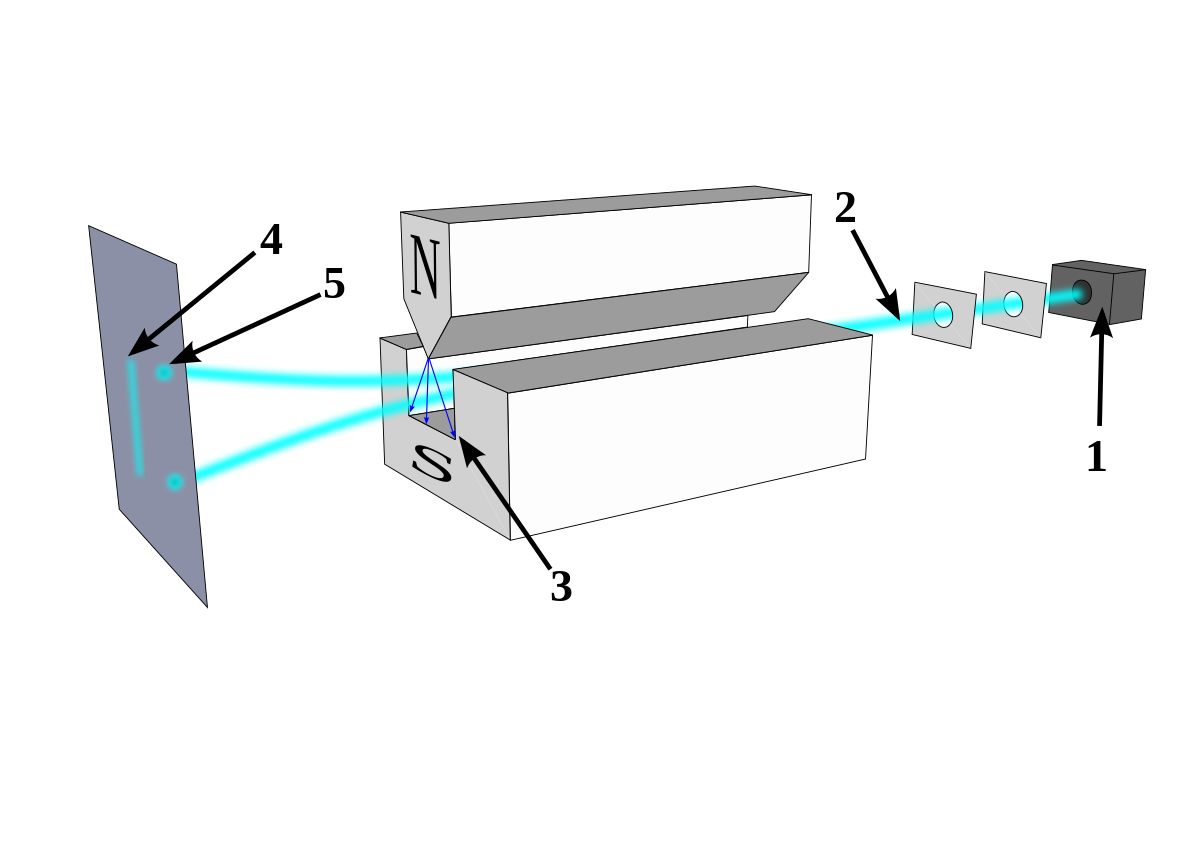
\includegraphics[width=8cm]{assets/stern_gerlach.png}
\end{center}
This experiment consisted of the measurement of the \textbf{magnetic dipole moment} of silver atoms. These silver atoms are sent as a stream (2) coming from an oven (1). Each atom is deflected from the path through an inhomogeneous magnetic field (3), and each atom is deflected from the path (5). This deflection is proportional to its dipole in the direction of the magnets. \\ \\
This experiment revealed no detection in the middle of the screen (4) but rather two sharp peaks at equal distances from the center (5). The quantity measured by the experiment is known in quantum mechanics as \textbf{spin}. \\ \\
In the case of a single measurement, for example, in the $z$-direction, it will result in two identical rays.

\begin{center}
	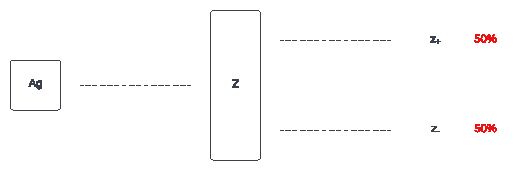
\includegraphics[width=10cm]{assets/one_z_measurement.pdf}
\end{center}
If the exact measurement is repeated for only one of the rays -- say $z_+$, then all the atoms are deflected again in the $+$ direction.

\begin{center}
	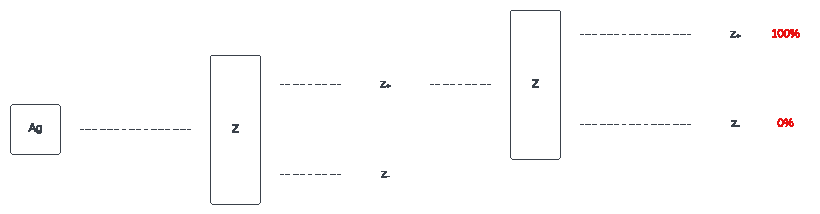
\includegraphics[width=11.5cm]{assets/two_z_measurements.pdf}
\end{center}
Finally, if the magnet is rotated and a $x$-direction measurement of the $z_+$ ray is made, another $z$-direction measurement, a 50-50 distribution. This puts the stability and the independence of the properties in question.

\begin{center}
	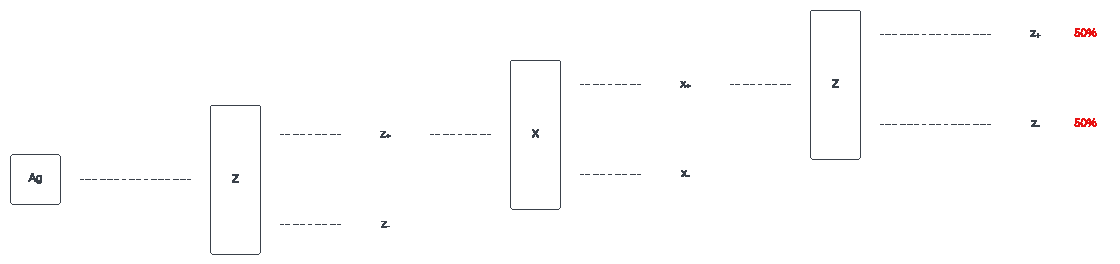
\includegraphics[width=12cm]{assets/z_x_z_measurements.pdf}
\end{center}

\subsection{Superposition}
Quantum superposition is a fundamental principle of quantum mechanics. It states that any two -- or more -- quantum states can be added together, and the result will be another valid quantum state. \\ \\
The question of whether a silver atom is in the state $| z_- \rangle$ or in the state $| z_+ \rangle$ are complementary to one another. They can be regarded as two answers to the same question -- i.e., the $Z$ measurement. \\ \\
If after performing an $X$ measurement, we want to know whether the silver atom is in a state $| x_+ \rangle$ or $| x_- \rangle$. Both are qual superpositions
\[ |x_+\rangle = \frac{1}{\sqrt{2}}|z_+\rangle + \frac{1}{\sqrt{2}}|z_-\rangle \]
\[ |x_-\rangle = \frac{1}{\sqrt{2}}|z_+\rangle - \frac{1}{\sqrt{2}}|z_-\rangle \]
No matter if we obtain one measurement or the other in the $Z$ measurement, the $X$-measurement either $| x_+ \rangle$ or $| x_- \rangle$ with equal probability. This is also known as a \textbf{quantum jump}.

\begin{center}
	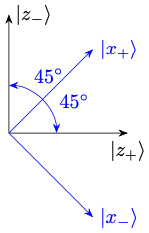
\includegraphics[width=2cm]{quantum_jump.png}
\end{center}

\subsection{Quantum Key Distribution}
We have seen that we can measure with certainty the same value in two consecutive measurements with the same basis. In other words, the interactions of a system with its environment become traceable. This traceability enables us to detect an eavesdropper in a \textbf{quantum cryptographic key agreement protocol}. \\ \\
The distribution of the key starts with \textit{Alice} using random measurements to encrypt the data. The encrypted photons are then sent to \textit{Bob}, which also uses random measurements to try and decrypt the data. After this process has terminated, \textit{Alice} sends the measurement basis she used to \textit{Bob} on a public channel. \textit{Bob} now takes the measurement basis and confronts it with his basis. The equal measurements are used as the \textbf{key}. \\ \\
If an eavesdropper, say \textit{Eve}, tries to intercept the message, she will need to guess the measurements for each photon. If the measurement is wrong, the system is disturbed. This means that \textit{Eve} has a probability of $1/4$ to be wrong in each stage. Thus, there is an almost 100\% probability of whether there was an eavesdropper.

\subsection{The Double-Slit Experiment}
If one shines a light onto a double slit, an interference pattern appears on the screen behind the double slit.

\begin{center}
	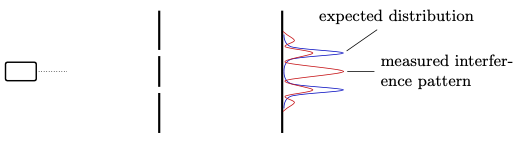
\includegraphics[width=10cm]{assets/double_slit.png}
\end{center}
If we were to measure the position of the photons on the screen (to the right of the image), an interference pattern would emerge. This means that single particles exhibit wave properties. However, if we look at the particles' paths, the interference pattern disappears.

\subsection{The Mach/Zehnder Interferometer}
The Mach/Zehnder interferometer can be considered a variant of the double-slit experiment.

\begin{center}
	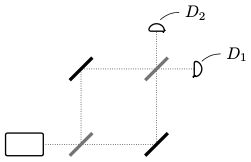
\includegraphics[width=5cm]{assets/interferometer.png}
\end{center}
If one sends single photons into the interferometer, the interference will occur, and the photons will be detected with certainty in detector $D_1$. \\ \\
In each \textbf{reflection}, the photon will pick up a phase shift of $\pi / 2$. Let us label the state of the photon moving to the \textbf{right} as $|1\rangle$, and the state of the photon moving \textbf{up} as $|2\rangle$. Their effect on \textbf{fully-reflecting mirrors} will then be:
\[ |1\rangle \mapsto i|2\rangle ~~~~~~~~ |2\rangle \mapsto i|1\rangle \]
While the effect on \textbf{semi-transparent mirrors} is:
\[ |1\rangle \mapsto \frac{1}{\sqrt{2}}(|1\rangle + i|2\rangle) ~~~~~~~~ |2\rangle \mapsto \frac{1}{\sqrt{2}}(|2\rangle + i|1\rangle) \]
Since we have these linear mappings, we can now track the photon through the interferometer. Since the emitter sends it to its right, the photon will start with a state of $|1\rangle$ --. Then we will have the following when hitting the \textbf{first semi-transparent mirror}:
\[ |1\rangle \mapsto \frac{1}{\sqrt{2}}(|1\rangle + i|2\rangle) \]
Now, the photon encounters a \textbf{fully-reflective mirror}, thus we need to apply the mappings to both $|1\rangle$ and $|2\rangle$ of the previous mapping:
\[ \frac{1}{\sqrt{2}}(|1\rangle + i|2\rangle) \mapsto \frac{1}{\sqrt{2}}(i|2\rangle + i \cdot i|1\rangle) \mapsto \frac{1}{\sqrt{2}}(i|2\rangle - |1\rangle) \]
Finally, the photon will again encounter a \textbf{semi-transparent mirror}. Thus, we will need to apply the mappings to both $|1\rangle$ and $|2\rangle$ again.
\begin{align*}
	\frac{1}{\sqrt{2}}(i|2\rangle - |1\rangle) &\mapsto \frac{1}{\sqrt{2}}\left(i\frac{1}{\sqrt{2}}(|2\rangle + i|1\rangle) - \frac{1}{\sqrt{2}}(|1\rangle + i|2\rangle) \right) \\
	&\mapsto \frac{1}{\sqrt{2}} \left( \frac{1}{\sqrt{2}}(i|2\rangle + i \cdot i|1\rangle) - \frac{1}{\sqrt{2}}(|1\rangle + i|2\rangle) \right) \\
	&\mapsto \frac{1}{\sqrt{2}} \left( \frac{1}{\sqrt{2}}(i|2\rangle - |1\rangle) - \frac{1}{\sqrt{2}}(|1\rangle + i|2\rangle) \right) \\
	&= -|1\rangle
\end{align*}
The photon, which now has state $-|1\rangle$, will be measured with certainty by detector D1.

\subsection{Quantum Bit}
To transfer a bit into the quantum world, we associate 0 and 1 with two orthogonal vectors:
\[ |0\rangle = \begin{pmatrix} 1 \\ 0 \end{pmatrix} ~~~~~~~~ |1\rangle = \begin{pmatrix} 0 \\ 1 \end{pmatrix} \]
A general quantum state can now be written as a superposition:
\[ |\psi\rangle = \alpha |0\rangle + \beta |1\rangle ~~~~~~~\text{with}~\alpha, \beta \in \mathbb{C};~\text{and}~|\alpha|^2 + |\beta|^2 = 1 \]
Measuring $|\psi\rangle$ in the standard basis will yield:

\begin{itemize}
	\item 0 -- With a probability of $|\alpha|^2$
	\item 1 -- With a probability of $|\beta|^2$
\end{itemize}

\subsubsection{Hadamard Gate}
Quantum circuits are composed of quantum gates which are \textbf{unitary maps}. The most important gate is the Hadamard gate. Which can be formalized as follows:
\[ H = \frac{1}{\sqrt{2}} \begin{pmatrix} 1 & 1 \\ 1 & -1 \end{pmatrix} \]
Which maps to the following superpositions:
\[ H|0\rangle = \frac{1}{\sqrt{2}}(|0\rangle + |1\rangle) ~~~~~~~~ H|1\rangle = \frac{1}{\sqrt{2}}(|0\rangle - |1\rangle) \]
Applying the Hadamard gate again will yield the standard basis vectors again.

\subsubsection{Square Root of NOT}
Another interesting gate is the following:
\[ F = \frac{1}{\sqrt{2i}} \begin{pmatrix} 1 & i \\ i & 1 \end{pmatrix} \]
When we apply this gate twice, we will obtain:
\[ F \cdot F = \begin{pmatrix} 0 & 1 \\ 1 & 0 \end{pmatrix} \]
In classical mechanics, no gate yields the not-gate this way. The gate $F$ has thus been called the "square root of NOT".

\subsection{Deutsch's Algorithm}
Given a function
\[ f : \{ 0, 1 \} \rightarrow \{ 0, 1 \} \]
We want to find out whether $f$ is constant and $f(0) \oplus f(1)$ is 0 or 1. In classical mechanics, we would have to query the function twice to get both answers. But there is another way to find out. First, we need to transform the black box into a \textbf{quantum black box}. Because of the unitarity of the quantum mechanical time evolution, the quantum box is \textbf{reversible}.

\begin{center}
	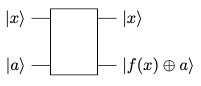
\includegraphics[width=4cm]{assets/deutsch.png}
\end{center}
This means that, if $a$ is 0, then $x$ is mapped to $|f(x)\rangle$ on the ouput wire. Moreover, if $a$ is 1, then $x$ is mapped to $\overline{|f(x)\rangle}$ -- which is the negation of $|f(x)\rangle$. \\ \\
If we were to put a superposition on the input wire and set $a$ to 0, we would obtain the following combined input:
\[ \frac{1}{\sqrt{2}}(|0\rangle + |1\rangle) \otimes |0\rangle = \frac{1}{\sqrt{2}} (|0\rangle \otimes |0\rangle + |1\rangle \otimes |0\rangle) \]
If:
\[ |0\rangle \otimes |0\rangle \mapsto |0\rangle \oplus |f(0)\rangle ~~~~~~~~ |1\rangle \otimes |0\rangle \mapsto |1\rangle \oplus |f(1)\rangle \]
Then, by linearly combining the two we obtain:
\[ \frac{1}{\sqrt{2}}(|0\rangle + |1\rangle) \otimes |0\rangle \mapsto \frac{1}{\sqrt{2}}(|0\rangle \oplus |f(0)\rangle + |1\rangle \oplus |f(1)\rangle \]
The resulting state is said to be \textbf{entangled}. This means that we cannot access information about $f(0)$ and $f(1)$ by merely measuring the output wire. However, if we also put a superposition on the second wire
\[ |a\rangle = \frac{1}{\sqrt{2}}(|0\rangle - |1\rangle) \]
Then we can expand the combined input as:
\begin{align*}
	& \frac{1}{\sqrt{2}}(|0\rangle + |1\rangle) \otimes \frac{1}{\sqrt{2}}(|0\rangle - |1\rangle) \\
	=~& \frac{1}{\sqrt{2}}(|0\rangle \otimes |0\rangle - |0\rangle \otimes |1\rangle + |1\rangle \otimes |0\rangle  - |1\rangle \otimes |1\rangle)
\end{align*}
Applying the gate to each summand, we obtain:
\[ \frac{1}{\sqrt{2}} \left( |0\rangle \otimes \big( |f(0)\rangle - \overline{|f(0)\rangle} \big) + |1\rangle \otimes \big( |f(1)\rangle - \overline{|f(1)\rangle} \big) \right) \]
If $f(0) = f(1)$, then:
\[ \frac{1}{\sqrt{2}}(|0\rangle + |1\rangle) \otimes \big( |f(0)\rangle - \overline{|f(0)\rangle} \big) \]
Otherwise:
\[ \pm \frac{1}{\sqrt{2}}(|0\rangle - |1\rangle) \otimes \big( |f(0)\rangle - \overline{|f(0)\rangle} \big) \]
If we now measure the standard basis of the output -- after having applied the Hadamard gate, this will yield:

\begin{center}
	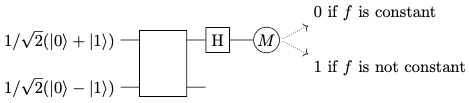
\includegraphics[width=9cm]{assets/deutsch2.png}
\end{center}
This algorithm does not allow us to retrieve more information. It does not yield the values of $f(0)$ or $f(1)$. What it yields is the result of $f(0) \oplus f(1)$.

\subsection{The Aspect/Gisin/Zelinger Experiments}
Quantum information processing is more than the fact that "a pair of Qbits is just one Qbit plus another Qbit". A striking manifestation is that other qualities arise when two entangled Qbits are independently measured. \\ \\
Imagine that -- inside of a preparation center -- pairs of Qbits (i.e., polarized photons) are generated and sent onto their respective paths to two parties -- \textit{Alice} and \textit{Bob}. What is sent to both \textit{Alice} and \textit{Bob} are two parts of the equal superpositions of $|0\rangle \otimes |0\rangle$ and $|1\rangle \otimes |1\rangle$. If \textit{Alice} and \textit{Bob} both measure in the standard basis -- i.e., $\{ |0\rangle, |1\rangle \}$, then they always receive the same output: a \textbf{perfect correlation}.

\subsubsection{Einstein/Podolsky/Rosen's Claim}
These three scientists, in 1935, claimed that quantum theory was \textbf{incomplete} and that it must be augmented by some "hidden parameters" that determine the measurement outcomes of all alternative measurements entirely.

\subsubsection{Bell's Claim}
Bell gave \textit{Alice} and \textit{Bob} more freedom. Now they could do measurements on a standard basis and other orthogonal bases. Bell claimed that EPR (Einstein/Podolsky/Rosen) is in doubt. There exist quantum correlations that go beyond the explanatory power of shared classical information. To prove it, Bell used a \textbf{singlet} and made \textit{Alice} and \textit{Bob} make measurements on different bases. \\ \\
Moreover, Bell discovered that measurement results are correlated; however, this correlation arises only upon measurement -- and not before it. This is known as \textbf{Bell non-locality}.











\section{Glossary}
\subsection{Magnetic Dipole Moment}
The magnetic dipole moment is a vector that represents the strength and orientation of a magnet or other object that produces a magnetic field (e.g., an electron).

\subsection{Singlet}
A singlet is a maximally-entangled state. However, this one has nicer transformation properties differently from other maximally-entangled states. For instance, a singlet written with respect to a general basis has the same form as the standard basis.

\end{document}

































